\documentclass{article}
\usepackage{amsmath}
\usepackage{graphicx}
\usepackage{subcaption}
\usepackage{setspace}
\usepackage[backend=bibtex,style=verbose-trad2]{biblatex}
\usepackage{siunitx}
\usepackage{multirow}
\usepackage{booktabs}
\usepackage{longtable}
\usepackage{rotating}
\usepackage{pgfplotstable}
\usepackage{listings}
\usepackage{color}
\usepackage{hyperref}
\usepackage{enumitem}

\begin{document}
\newpage
\pagenumbering{arabic}

\section{Analysis}
\subsection{Background}
Mr Myslov is a teacher at Tonbridge School, and currently runs the school chess club. Seldomly, a field day event will be held, in which the club convenes together, playing a chess, or another variant, tournament. This year, Mr Myslov has decided to instead, hold a tournament around another board game, namely laser chess, providing a deviation yet retaining the same familiarity of chess. However, multiple physical sets of laser chess have to be purchased for the entire club to play simultaneously, which is difficult due to it no longer being manufactured. Thus, I have proposed a solution by creating a digital version of the game.

\subsubsection{Game Description}
Laser Chess is an abstract strategy game played between two opponents. The game differs from regular chess, involving a 10x8 playing board arranged in a predefined condition. The aim of the game is to position your pieces such that your laser beam strikes the opponents Pharoah (the equivalent of a king). Pieces include:

\begin{enumerate}
\item Pharoah
    \begin{itemize}[label=(-)]
    Equivalent to the king in chess
    \end{itemize}
\item Scarab
    \begin{itemize}[label=(-)]
    2 for each colour
    Contains dual-sided mirrors, capable of reflecting a laser from any direction
    Can move into an occupied adjacent square, by swapping positions with the piece on it (even with an opponent’s piece)
    \end{itemize}
\item Pyramid
    \begin{itemize}[label=(-)]
    7 for each colour
    Contains a diagonal mirror used to direct the laser
    The other 3 out of 4 sides are vulnerable from being hit
    \end{itemize}
\item Anubis
    \begin{itemize}[label=(-)]
    2 for each colour
    Large pillar with one mirrored side, vulnerable from the other sides
    \end{itemize}
\item Sphinx
    \begin{itemize}[label=(-)]
    1 for each colour
    Piece from which the laser is shot from
    Cannot be moved
    \end{itemize}
\end{enumerate}

On each turn, a player may move a piece one square in any direction (similar to the king in regular chess), or rotate a piece clockwise or anticlockwise by 90 degrees. After their move, the laser will automatically be fired. It should be noted that a player’s own pieces can also be hit by their own laser. As in chess, a three-fold repetition results in a draw. Players may also choose to forfeit or offer a draw.

\subsection{Client Interview}

\subsection{Current solutions}
Current free implementations of laser chess that are playable online are limited, seemingly only available on \url{https://laser-chess.com/}.

\begin{figure}
    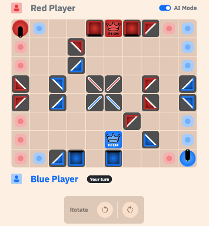
\includegraphics[width=\linewidth]{assets/laserchesscom.png}
    \caption{Online implementation on laser-chess.com}
    \label{fig:laserchesscom}
\end{figure}

The game is hosted online and is responsive and visually appealing, with pieces easy to differentiate and displaying their functionality clearly. It also contains a two-player mode for playing between friends, or an option to play against a functional CPU bot. However, the game lacks the following basic functionalities that makes it unsuitable for my client’s requests:

\begin{itemize}
\item No replay options (going through pass moves)
    \begin{itemize}
    \item A feature to look through previous moves is standard in any online chess implementation
    \item My client requires this feature as it is an essential tool in learning from past games and to aid in analyzing the course of a game and opponent’s thought process
    \end{itemize}
\item No option to save and load previous games
    \begin{itemize}
    This QOL feature allows games to be continued on if they cannot be finished in one sitting
    \end{itemize}
\item Internet connection required
    \begin{itemize}
    My client has specifically requested an offline version as the game will predominantly played in settings where a connection might not be available (i.e. on a plane)
    \end{itemize}
\item Unable to change board configuration
    \begin{itemize}
    The version of laser chess named Khet contains different starting board configurations, each offering a different style of play
    Our design will aim to append the missing feature from this website while learning from their valid UI design.
    \end{itemize}
\end{itemize}

\subsection{Objectives}

\end{document}